\documentclass[../main.tex]{subfiles}

\graphicspath{{\subfix{../img/}}}

\begin{document}
   \part{Logica Descrittiva}

   \chapter{Logica}

   \section{Intuizioni}
   La FOL con la sua espressività permette di usare:
   \begin{itemize}
      \item costanti
      \item variabili libere
      \item simboli di funzioni
      \item \dots
   \end{itemize}
   Ma nella maggior parte delle applicazioni dell'informatica questa espressività non è richiesta.\\
   La grande espressività della FOL è motivita dal suo uso, ma si porta dietro dei costi di analisi molto elevati.\\
   Il linguaggio della FOL non ha struttura, risulta quindi appiattito, questo nonostante elementi diversi formalizzino intuizioni diverse.\\
   La FOL (e la PL) nella loro semantica hanno lo scopo di dare giudizi riguardanti dei fatti e quindi anche selle conseguenze sui fatti risultati veri.\\
   Per lo stesso motivo FOL e PL non forniscono alcuno strumento per ragionare sui fatti perchè codificati in formule atomiche, il predicato $P(t_1, \dots , t_n)$ viene usato solo per determinare quando lo stato è vero o falso.
   \begin{center}
      \begin{tabular}{c c c}
         $I \models t_1 = t_2[a]$ & iff & $I(t_1)[a] = I(t_2)[a]$\\
         $I \models P(t_1, \dots ,t_n)[a]$ & iff & $< I(t_1)[a], \dots, I(t_n)[a] > \in I(P) >$
      \end{tabular}
   \end{center}

   \subsection{Da FOL a logica descrittiva (DL)}
   \textbf{Espressività:} l'espressività è molto limitata perchè non abbiamo variabili libere, simboli di funzione e abbiamo solo predicati binari come simboli primitivi.
   \spazio
   \textbf{Decidibilità:} dobbiamo ridurre i domini in domini finiti e usare l'assunzione dei nomi univoci, lo standard sono le pratiche dei domini relazionali.
   \spazio
   \textbf{Mancanza di struttura:} per questa mancanza della FOL vengono esplicitate varie distinzioni:
   \begin{itemize}
      \item Come sono costrite le classi.
      \item Classi e ruoli (predicati unari vs binari).
      \item Schemi contro schemi popolati (TBox e ABox).
      \item Ragionamento schematico  (knowledge-level) contro ragionamento ground  (data-level).
   \end{itemize}
   \textbf{Scopo:} lo scopo della DL non è ragionare su cosa è vero ma ragionare sui fatti e sulle loro componenti.

   \section{Due logiche}
   \begin{itemize}
      \item \textbf{Conoscenze:} 
         \begin{itemize}
            \item Linguaggio naturale: informazioni e principi.
            \item Computer Science: il nome delle classi, il nome delle relazioni.
            \item Logica: predicati simbolici, qunatificatori universali e di esistenza.
         \end{itemize} 
      \item \textbf{Dati:}
         \begin{itemize}
            \item Linguaggio naturale: informazioni fattuali o calcolo.
            \item Computer Science: valori dei dati, enità e proprietà degli oggetti.
            \item Logic: costanti, termini ground e formule ground.
         \end{itemize}
   \end{itemize}
   L'usuale linguaggio è diviso in due insiemi ma collegati tra di loro:
   \begin{itemize}
      \item \textbf{TBox - la logica della conoscenza:} il linguaggio e la logica usati per specificare e ragionare sugli schemi usati per modellare i dati.\\
         Le TBox mappano direttamente in modelli Extended Entity-relationship (EER), relazioni dei DB e Knowledge Graphs (KG).
      \item \textbf{ABox - la logica dei dati:} il linguaggio e la logica usati per memorizzare e ragionare sui dati, si mappa sui dati contenuti nei DB e nei KG.
   \end{itemize}
   \textbf{T} significa \textbf{Terminologia} mentre \textbf{A} vuol dire \textbf{Asserzione}, sono collegati perchè le asserzioni fatte nelle ABox sfrutta la terminologia definita dalle TBox.\\
   In questo corso vedremmo la logica descrittiva $\mathcal{ALC}$, ovvero la DL la cui parte proposizionele corrisponde perfettamente alla PL.

   \section{Sintassi TBox}
   \textbf{Alfabeto:} un alfabeto è composto dai seguenti simboli:
   \begin{itemize}
      \item Simboli non logici: nomi di concetti (classi) quindi come persone, animali, cose \dots
      \item Simboli logici: 
         \begin{itemize}
            \item $\sqcap$ congiunzione, $\sqcup$ disgiunzione e $\lnot$ negazione di concetto.
            \item $\top$ dominio di interpretazione e $\perp$ insieme vuoto.
         \end{itemize}
   \end{itemize}
   \textbf{Conectto:} è un insieme di entità, la relazione formalizzata nei DB.

   Di seguito parleremo di concetto (interpretazione) intendendo il nome del concetto (linguaggio). 
   \spazio
   \textbf{Ruolo:} un lafabeto contiene i seguenti simboli:
   \begin{itemize}
      \item Simboli non logici: nomi di ruoli (relazioni) $R_1, R_2, \dots , R_n$.
      \item Simboli logici: $\forall$ e $\exists$.
   \end{itemize}

   \subsubsection{Esempio di ruoli}
   Consideriamo i seguenti concetti e nomi:
   \begin{itemize}
      \item Nomi concetti:Vehicle, Boat, Bicycle, Car, Device, Wheel, Engine, Axle, Rotation, Water, Human, Driver, Adult, Child.
      \item Nomi ruoli: hasPart, poweredBy, capableOf, travelsOn, controls.
   \end{itemize}
   Formalizziamo una serie di frasi in linguaggio naturale.
   \begin{enumerate}
      \item Those vehicles that have wheels and are powered by an engine.
      \item Those vehicles that have wheels and are powered by a human.
      \item Those vehicles that travel on water.
      \item Those objects which have no wheels.
      \item Those objects which do not travel on water.
      \item Those devices that have an axle and are capable of rotation.
      \item Those humans who control a vehicle.
      \item The drivers of cars.
   \end{enumerate}
   Le trasposizioni in DL sono:
   \begin{enumerate}
      \item Vehicle$\sqcap \exists$hasPart.Wheel$\sqcap \exists$poweredBy.Engine
      \item Vehicle$\sqcap \exists$hasPart.Wheel$\sqcap \exists$poweredBy.Human
      \item Vehivle$\sqcap \exists$travelsOn.Water
      \item $\forall$hasPart.$\lnot$Wheel
      \item $\forall$ travelsOn.$\lnot$Water
      \item Device$\sqcap \exists$hasPart.Axle$\sqcap \exists$capableOf.Rotation
      \item Human$\sqcap \exists$controls.Vehicle
      \item Driver$\sqcap \exists$controls.Car
   \end{enumerate}
   \vspace{2em}
   \textbf{Descrizione concettuale:} dato un insieme di nomi di concetti \textbf{C} e un insieme di nomi di ruoli \textbf{R}, l'insieme delle descrizioni dei concetti su \textbf{C} e \textbf{R} è definito come:
   \begin{itemize}
      \item Ogni nome di un concetto è una descrizione di concetto.
      \item $\top$ e $\bot$ sono descrizioni di concetti.
      \item Se C e D sono due concetti e $r$ il nome di un ruolo, allora le seguenti formule sono descrizioni di concetti:
      \begin{itemize}
         \item C $\sqcap$ D
         \item C $\sqcup$ D
         \item $\lnot$ C
         \item $\exists$ $r$.C
         \item $\forall$ $r$.C
      \end{itemize} 
   \end{itemize}
   La descrizione concettuale non esprime le relazioni in un DB ma le assunzioni che si fanno per fare il design di un DB.
   \spazio
   \textbf{Dominio di interpretazione:} un dominio di interpretazione in DL è un insieme i cui elementi sono chiamati individui o oggetti, nel seguente modo:
   \begin{itemize}
      \item Per ogni nome di concetto gli elementi appartenenti alla sua estensione sono parte del dominio.
      \item Per ogni nome di ruolo gli elementi (coppie ordinate di elementi) appartenenti alla sua estensione sono parte del dominio.
   \end{itemize}
   \vspace{2em}
   \textbf{Interpretazione TBox:} dato un insieme di nomi di concetti \textbf{C} e un insieme di nomi di ruoli \textbf{R}; dato un dominio $\Delta ^\prime$, un interpretazione $I=(\Delta^\prime, \cdot^\prime)$ è composta dal dominio con una funzione di mappatura che:
   \begin{itemize}
      \item Associa ogni nome di concetto C $\in$ \textbf{C} ad un insieme C$^\prime \subseteq \Delta^\prime$.
      \item Associa ogni nome di ruolo $r \in$\textbf{R} ad un insieme $r^\prime \subseteq \Delta^\prime \times \Delta^\prime$.
      \item Associa descrizioni di concetti composti nel seguente modo:
      \begin{itemize}
         \item $\top^\prime = \Delta^\prime$
         \item $\bot^\prime = \emptyset$
         \item $(C \sqcap D)^\prime = C^\prime \cap D^\prime$
         \item $(C \sqcup D)^\prime = C^\prime \cup D^\prime$
         \item $\lnot C^\prime = \Delta^\prime \backslash C^\prime$
         \item $(\exists r.C) = \{ d \in \Delta^\prime | \text{esiste una } e \in \Delta^\prime \text{con } (d,e) \in r^\prime \text{ e } e \in C^\prime\}$
         \item $(\forall r.C) = \{ d \in \Delta^\prime | \text{per tutte le } e \in \Delta^\prime \text{se } (d,e) \in r^\prime \text{ allora } e \in C^\prime\}$
      \end{itemize} 
   \end{itemize}

   \section{Teorie TBox}
   \textbf{Concetto di inclusione:} un concetto di inclusione è un'espressione della seguente forma:
   \begin{center}
      $C \sqsubseteq D$
   \end{center}
   dove C e D sono descrizioni di concetti. $C \sqsubseteq D$ va letto come "C è sussunta da D".

   \subsubsection{Esempio}
   Consideriamo i seguenti concetti e nomi:
   \begin{itemize}
      \item Nomi concetti:Vehicle, Boat, Bicycle, Car, Device, Wheel, Engine, Axle, Rotation, Water, Human, Driver, Adult, Child.
      \item Nomi ruoli: hasPart, poweredBy, capableOf, travelsOn, controls.
   \end{itemize}
   Formalizziamo una serie di frasi in linguaggio naturale.
   \begin{enumerate}
      \item Boats have no wheels.
      \item Cars and bicycles do not travel on water.
      \item Drivers of cars are adults.
      \item Humans are not vehicles.
      \item Wheels or engines are not humans.
      \item Humans are either adults or children.
      \item Adults are not children.
   \end{enumerate}
   Le trasposizioni in DL sono:
   \begin{enumerate}
      \item Boat$\sqsubseteq \forall$hasPart.$\lnot$Wheel
      \item Car$\sqcup$Bicycle$\sqsubseteq \forall$travelsOn.$\lnot$Water
      \item Driver$\sqcap \exists$controls.Car$\sqsubseteq$Adult
      \item Human$\sqsubseteq \lnot$Vehicle
      \item Wheel$\sqcup$Engine$\sqsubseteq \lnot$Human
      \item Human$\sqsubseteq$Adult$\sqcup$Child
      \item Adult$\sqsubseteq \lnot$Child
   \end{enumerate}
   \vspace{2em}
   \textbf{Soddisfabilità dell'inclusione dei concetti:} sia \textbf{C} un insieme di nomi di concetti e \textbf{R} un insieme di nomi di ruoli, allor adato un dominio $\Delta^\prime$ e un'interpretazione $I = (\Delta^\prime, \cdot^\prime)$ abbiamo che:
   \begin{center}
      se $C^\prime \subseteq D^\prime$ allora $I$ è un modello di $C \sqsubseteq D$
   \end{center}
   dove C e D sono descrizionali concettuali.
   \spazio
   \textbf{TBox:} una TBox è un insieme finito di inclusioni concettuali, come un insieme finito di espressioni $C \sqsubseteq D$, dove C e D sono nomi di concetti (che possibilmente coinvolgono concetti composti).
   
   \subsubsection{Esempio}
   Consideriamo la descrizione concettuale "Dogs are Computer Science professors", che in DL diventa Dog $\sqsubseteq$ CS\_Professor.\\
   Possiamo dimostrare l'insoddisfacibilità di questa frase con una TBox:
   \begin{equation*}
      \T=
      \begin{cases}
         CS\_Professor \sqsubseteq Professor\\
         Professor \sqsubseteq Person\\
         Person \sqsubseteq \lnot Dog
      \end{cases}
   \end{equation*}
   \spazio
   \textbf{Modello per TBox:} sia \textbf{C} un insieme di nomi di concetti e \textbf{R} un insieme di nomi di ruoli, dato $\Delta^\prime$ e la sua interpretazione $I = (\Delta^\prime, \cdot^\prime)$, C e D descrizioni concettuali allora se $C^\prime \subseteq D^\prime$ per ogni $C \sqsubseteq D \in \T$ vuol dire che $I$ è un moodello per $\T$.
   \spazio
   \textbf{Definizione di concetto:} una definizione di concetto è un'espressione della seguente forma:
   \begin{center}
      $C \equiv D$ se e solo se $C \sqsubseteq D$ e $D \sqsubseteq C$.
   \end{center}
   dove C e D sono descrizioni concettuali e $C \equiv D$ va letto come "C è equivalente a D".

   \subsubsection{Esempio}
   Consideriamo i seguenti concetti e nomi:
   \begin{itemize}
      \item Nomi concetti:Vehicle, Boat, Bicycle, Car, Device, Wheel, Engine, Axle, Rotation, Water, Human, Driver, Adult, Child.
      \item Nomi ruoli: hasPart, poweredBy, capableOf, travelsOn, controls.
   \end{itemize}
   Formalizziamo una serie di frasi in linguaggio naturale.
   \begin{enumerate}
      \item Cars are exactly those vehicles that have wheels and are powered by an engine
      \item Bicycles are exactly those vehicles that have wheels and are powered by a human
      \item Boats are exactly those vehicles that travel on water
      \item Wheels are exactly those devices that have an axle and are capable of rotation
      \item Drivers are exactly those humans who control a vehicle
   \end{enumerate}
   Le trasposizioni in DL sono:
   \begin{enumerate}
      \item Car$\equiv$Vehicle$\sqcap \exists$hasPart.Wheel$\sqcap \exists$poweredBy.Engine
      \item Bicyle$\equiv$ Vehicle$\sqcap \exists$hasPart.Wheel$\sqcap \exists$poweredBy.Human
      \item Boat$\equiv$ Vehicle$\sqcap \exists$travelsOn.Water
      \item Wheel$\equiv$Device$\sqcap \exists$hasPart.Axle$\sqcap \exists$capableOf.Rotation
      \item Driver$\equiv$Human$\sqcap \exists$controls.Vehicle
   \end{enumerate}
   \vspace{2em}
   \textbf{TBox definita:} una TBox è definita se soddiafa le seguenti proprietà:
   \begin{itemize}
      \item Ogni concetto può apparire al più una volta nel lato sinistro di una definizione.
      \item Sono presenti solo equivalenze concettuali $(C \equiv D)$.
      \item E' aciclica quindi non esistono definizioni del tipo $C \equiv C$.
   \end{itemize} 
   \subsubsection{Esempio}
   \begin{equation*}
      \T=
      \begin{cases}
         Person \equiv \exists hasname.String \sqcap \forall HasJob.Organization\\
         Woman \equiv Person \sqcap  Female\\
         Man \equiv Person \sqcap  \lnot Woman\\
         Mother \equiv Woman \sqcap  \exists hasChild.Person\\
         Father \equiv Man \sqcap  \exists hasChild.Person\\
         Parent \equiv Father \sqcup Mother
      \end{cases}
   \end{equation*}
   \spazio
   \textbf{Unfolding di concetti:} un concetto è unfolded se tutte le sue componenti hanno una definizioni.
   \spazio
   \textbf{TBox unfolding:} una TBox $\T$ può essere unfolded in una TBox $\T^\prime$ se tutti i suoi concetti sono unfolded.

   \section{Sintassi ABox}
   \textbf{Asserzione:} un asserzione è un espressione del tipo:
   \begin{itemize}
      \item C(a) asserzione di concetto
      \item r(a,b) asserzione di ruolo
   \end{itemize}
   dove a e b sono individui, C è un concetto (possibilmente composto) e r è il nome di un ruolo.
   \spazio
   \textbf{Interpertazione ABox:} sia \textbf{C} un insieme di nomi di concetti e \textbf{R} un unsieme di nomi di ruoli allora l'interpretazione di un'asserzione è definita come:
   \begin{itemize}
      \item $(C(a))^\prime = a^\prime \in C^\prime$
      \item $(r(a, b))^\prime = (a^\prime,b^\prime) \in r^\prime$
   \end{itemize}
   dove C è un concetto (possibilmente composto) e $r$ il nome di un ruolo.

   \section{Teorie ABox}
   \textbf{ABox:} un ABox è un insieme finito di asserzioni di concetti o asserzioni di ruoli, come un insieme finito di espressioni del tipo :
   \begin{itemize}
      \item C(a) asserzione di concetto
      \item r(a,b) asserione di ruolo
   \end{itemize} 
   dove a,b sono nomi individuali, C è un concetto composto e r è il nome di un ruolo.
   \spazio
   \textbf{Modello di un ABox:} sia \textbf{C} un insieme di nomi di concetti e \textbf{R} un insieme di nomi di ruoli.\\
   Un modelloo di un ABox è un'interpretazione che soddisfa ogni asserzione nell'ABox.\\
   L'interpetazione deve:
   \begin{itemize}
      \item $I$ soddisfa un'asserzione di concetto $C(a)$ se $a^\prime \in C^\prime$.
      \item $I$ soddisfa un'asserzione di ruolo $r(a,b)$ se $(a^\prime, b^\prime) \in r^\prime$. 
   \end{itemize}
   \vspace{2em}
   \textbf{Espansione di concetti:} sia $\T$ una TBox definita e $\A$ un ABox.\\
   Sia $C$ un concetto definito in $\T$ come $C \equiv C^\prime$ e occorrente in $\A$, sia poi $a$ un individuo occorrente in $\A$ allora $C^\prime (a)$, l'espansione di $C(a)$ rispetto a $\T$, è ottenibile sostituendo $C$ con $C^\prime$.
   \spazio
   \textbf{Espansione di ABox rispetto ad una TBox:} applicando l'espansione a tutti i concetti nella ABox e definiti nella TBox la nuova Abox $\A^\prime$ risultante è chiamata espansione di $\A$ rispetto a $\T$.

   \subsubsection{Esempio}
   Date le Tbox e ABox:
   \begin{equation*}
      \T=
      \begin{cases}
         Mother \equiv Female \sqcap \exists hasChild.Person\\
         Female \equiv Person \sqcap \lnot Male
      \end{cases}
   \end{equation*}
   \begin{equation*}
      \A=
      \begin{cases}
         Mother(Anna)
      \end{cases}
   \end{equation*}
   L'estensione di $\A$ rispetto a $\T$ é:
   \begin{equation*}
      \T^\prime=
      \begin{cases}
         Mother(Anna)\\
         Female(Anna)\\
         \exists hasChild.Person(Anna)\\
         Person(Anna)\\
         \lnot Male(Anna) 
      \end{cases}
   \end{equation*}
   \spazio
   \textbf{Conoscenze di base:} una conoscenza di base $\mathcal{K} = (\T,\A)$ è una tupla composta da una TBox $\T$ ed una ABox $\A$.
   \spazio
   \textbf{Modello di una base di conoscenza:} un interpretazione $I$ è un modello per una conoscenza di base $\mathcal{K} = (\T,\A)$ se è un modello sia per $\T$ e per $\A$.

   \chapter{Modeling}
   \section{Principali risultati teorici}
   DL è una specie di zucchero sintattico per un sottoinsieme di FOL, questo sottoinsieme è ristretto a termini binari, unari e nessun simbolo di funzione.
   \spazio
   \textbf{Da DL a FOL:} sia $T_{DF(X)}$ una funzione di traduzione da DL a FOL, abbiamo quindi le seguenti formule:
   \begin{itemize}
      \item $T_{DF(X)}(C) = C(x)$
      \item $T_{DF(X)}(C \sqcap D) = T_{DF(X)}(C) \land T_{DF(X)}(D)$
      \item $T_{DF(X)}(C \sqcup D) = T_{DF(X)}(C) \lor T_{DF(X)}(D)$
      \item $T_{DF(X)}(\exists r.C) = \exists y.r(x, y) \land TDF(y)(C)$
      \item $T_{DF(X)}(\forall r.C) = \forall y.r(x, y) \implies TDF(y)(C)$
   \end{itemize}
   Possimao avere le seguenti traduzioni:
   \begin{itemize}
      \item $T_{DF} (C \sqsubseteq D) = \forall x.(T_{DF}(x)(C) \implies T_{DF(x)}(D))$, per tutte le inclusioni concettuali in $\T$
      \item $T_{DF} (C(a)) = T_{DF(x)}(C[a/x])$, con $C(a) \in \A$
      \item $TDF (r(a, b)) = r(a, b)$, con $r(a,b) \in \A$
   \end{itemize}
   Sia ora $\mathcal{K}= (\T,\A)$ una knowledge base in DL con $T_{DF}(\T)$ e $T_{DF}(\A)$ rispettivamente gli insiemi di tutte le traduzioni delle inclusioni logiche $\T$ e asserzioni $\A$, abbiamo allora i seguenti teoremi:
   \begin{itemize}
      \item $\mathcal{K}$ è soddisfacibile se e solo se $T_{DF}(\T) \land T_{DF}(\A)$ è soddisfacibile.
      \item $C \sqsupseteq_\T D$ se e solo se è valida la seguente formula:
         \begin{equation*}
            T_{DF(\T)} \implies \forall x.(T_{DF(x)}(C) \implies T_{DF(x)}(D))
         \end{equation*}
      \item $a$ è un'istanza di $C$ rispetto a $\T$ se e solo se la seguente formula è valida:
         \begin{equation*}
            (T_{DF}(\T) \land T_{DF}(C)) \implies T_{DF(x)}(C[a/x])
         \end{equation*}
   \end{itemize}
   \vspace{2em}
   \textbf{Ragionamento in DL:} per poter applicare degli algoritmi di ragionamento su delle teorie (TBox e ABox) in DL dobbiamo prima tradurle in FOL e successivamente usare i Tableaux per verificare la validità ecc \dots della formula in FOL che abbiamo.
   \subsubsection{Esempio}
   Traduzione TBox dal linguaggio naturale prima in DL poi in FOL
   \begin{enumerate}
      \item A teacher is a person who teaches a course
      \item A student is a person who attends a course
      \item Students do not teach
   \end{enumerate}
   \begin{minipage}{0.5\textwidth}
      \textbf{Traduzioni in DL}
      \begin{enumerate}
         \item $Teacher \equiv Person \sqcap \exists teaches.Course$
         \item $Student \equiv Person \sqcap \exists attends.Course$
         \item $\exists teaches. \top \sqsubseteq \lnot Student$
      \end{enumerate} 
   \end{minipage}
   \begin{minipage}{0.5\textwidth}
      \textbf{Traduzioni in FOL}
      \begin{enumerate}
         \item $\forall x.(Teacher(x) \equiv Person(x) \land \exists y .(teaches(x,y) \land Course(y)))$
         \item $\forall x.(Student(x) \equiv Person(x) \land \exists y .(attends(x,y) \land Course(y)))$
         \item $\forall x.(\exists y.teaches(x,y) \supset \lnot Student(x))$
      \end{enumerate}
   \end{minipage}
   \spazio
   \textbf{Semantica del mondo chiuso:} è una metodologia di interpretazione tipica dei DB, se un elemento non è presente nel DB si assume sia falso.\\
   Permette quindi un solo modello quello in cui tutto ciò conosciuto è vero e tutto quello non conosciuto è falso.
   \spazio
   \textbf{Semantica del mondo aperto:} interpretazione tipica dei KG e delle Abox in cui non possiamo fare assunzioni su ciò che non conosciamo.\\
   Permette quindi molteplici modelli in cui ciò che non conosciamo può essere sia vero che falso.
   \subsubsection{Esempio}
   Prendiamo in esame la seguente base di conoscenza $\mathcal{K}=(\T,\A)$:
   \begin{gather*}
      \T=
      \begin{cases}
         Mother \equiv Female \sqcap \exists hasChild.Person
      \end{cases}\\
      \A=
      \begin{cases}
         Mother(Anna)\\
         hasChild(Anna, Bob)
      \end{cases}
   \end{gather*}
   \begin{itemize}
      \item Per la semantica del mondo chiuso Anna ha solo Bob come figlio.
      \item Per la semantica del mondo aperto Anna ha almeno Bob come figlio, potrebbe averne più come anche solo Bob.
   \end{itemize}
   
   \section{Da semi-formale a formale}
   \subsection{Modelo ER}
   Un ER descrive cose correlate tra di loro nel nostro dominio di conoscenza attraveso classi/entità e relazioni che collegano tra di loro le classi/entità.\\
   L'ER quindi non è altro che un modello astratto che definisce dati o informazioni  sulla struttura dei dati.
   \begin{center}
      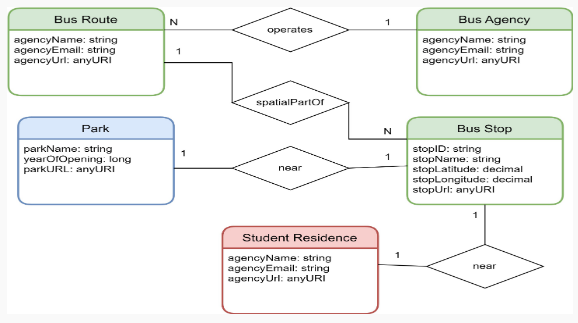
\includegraphics[scale=0.7]{ER_example.png}
   \end{center}

   \subsection{Modello EER}
   EER sta per Extended ER questo perchè partiamo da tutti i concetti definiti nei diagrammi ER, ai quali però aggiungiamo i concetti di sotto/super classe con la relazione "\textbf{is-a}".\\
   Una super classe è un'entità/classe che può essere divisa in più sotto classi e una sotto classe eredita le proprietà della sua super classe.\\
   Si possono adottare due metodi per creare super/sotto classi.
   \begin{enumerate}
      \item \textbf{Generalizzazione:} avendo un gruppo di sotto classi si cercano gli attributi che hanno in comune e con quelli si crea una super classe.
      \item \textbf{Specializzazione:} con una super classe classe si cerca di identificare un sottoinsieme di entità che hanno alcune caratteristiche diverse.
   \end{enumerate}
   \begin{center}
      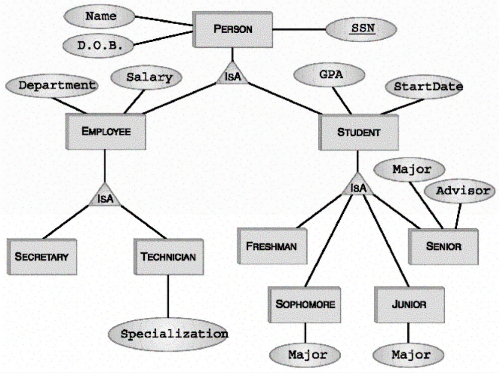
\includegraphics[scale=0.7]{EER_example.png}
   \end{center}
   \vspace{2em}
   Vediamo ora cosa vuol dire ontologia, questo termine ha significati differenti in base all'ambito in cui ci si trova.
   \spazio
   \textbf{Ontologia nella filosofia:} la disciplina che si occupa di dare un significato alla natura e alla struttura della realtà.
   \spazio
   \textbf{Ontologia in informatica:} è un tipo speciale di oggetto contenente informazioni oppure di artifatto prodotto dalla computazione.
   \begin{itemize}
      \item Modella formalmente la struttura di un sistema come le entità rilevanti e le relazioni che vengono scoperte.
   \end{itemize}

   \chapter{Ragionamento}
   \section{Problemi di ragionamento con le TBox}
   I principali problemi quando si opera con le TBox sono 4:
   \begin{enumerate}
      \item \textbf{Soddisfacibilità:} un concetto $C$ è soddisfacibile rispetto a $\T$ se esiste un modello $I$ di $\T$ tale che $C_I$ sia non vuoto, in questo caso possiamo anche dire che $I$ è un modello per $C$.
      \item \textbf{Sussunzione:} un concetto $C$ è sussunto da un concetto $D$ rispetto a $\T$ se $C^\prime \subseteq D^\prime$ per ogni modello $I$ di $\T$, in questo caso possiamo scrivere $C \sqsubseteq_\T D$ oppure $T \models C \sqsubseteq D$.
      \item \textbf{Equivalenza:} due concetti $C$ e $D$ sono equivalenti rispetto a $\T$ se $C^\prime = D^\prime$ per ogni modello $I$ di $\T$, in questo caso possiamo scrivere $C \equiv_\T D$ oppure $\T \models C \equiv D$.
      \item \textbf{Disgiunzione:} due concetti $C$ e $D$ sono disgiunti rispetto a $\T$ se $C^\prime \cap D^\prime = \emptyset$ per ogni modello $I$ di $\T$, in questo caso scriveremo $C \bot D$.
   \end{enumerate}
   E' possibile notare che se due concetti non si sussumono a vicenda e non sono disgiunti vuol dire che, a livello insiemistico, sono parzialmente sovvrapposti.
   \spazio
   \textbf{Consistenza di concetti:} un concetto $C$ è consistente con riferimento a $\T$ se esiste qualche interpretazione che soddisfa l'assioma $\T \cup C$ tale che $C$ sia un insieme non vuoto in quell'interpretazione, un concetto non vuoto viene detto soddisfacibile, insiddisfacibile altrimenti.
   
   \subsubsection{Esempio}
   Consideriamo la TBox:
   \begin{equation*}
      \T=
      \begin{cases}
         Undergraduate \sqsubseteq \lnot Teach\\
         Bachelor \equiv Student \sqcap Undergraduate\\
         Master \equiv Student \sqcap \lnot Undergraduate\\
         PhD \equiv Master \sqcap Research\\
         Assistant \equiv PhD \sqcap Teach\\
      \end{cases}
   \end{equation*}
   \begin{center}
      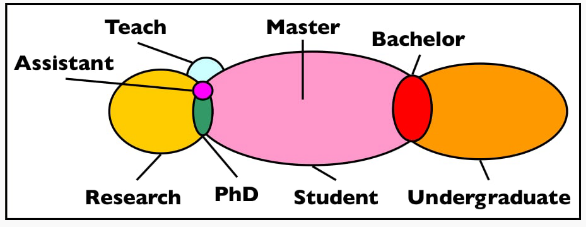
\includegraphics[scale=0.5]{venn_example.png}
   \end{center}
   Proviamo a vedere se il seguente fatto è consistente/soddisfacibile:
   \begin{equation*}
      \T \models Bachelor \sqcap PhD
   \end{equation*}
   Per provare che è falsa iniziamo a sostituire Bachelor e Phd con le definizioni che ho nella TBox fino a che non trovo un insieme vuoto.
   \begin{align*}
      &Bachelor \sqcap PhD\\
      &\equiv (Student \sqcap Undergraduate) \sqcap (Master \sqcap Research)\\
      &\equiv (Student \sqcap Undergraduate) \sqcap ((Student \sqcap \lnot Undergraduate) \sqcap Research)\\
      &\equiv Student \sqcap \textbf{Undergraduate} \sqcap \lnot \textbf{Undergraduate} \sqcap Research\\
      &\equiv Student \sqcap \bot \sqcap Research
   \end{align*}
   \spazio
   \textbf{Sussunzione di concetti:} un concetto $C$ è sussunto da un concetto $D$ se in ogni modello di $\T$ l'insieme denotato da $C$ è sottoinsieme dell'insieme denotato da $D$.
   \spazio
   \textbf{Equivalenza di concetti:} è spesso definita usando la sussunzione dei concetti:
   \begin{equation*}
      \T \models C \equiv D\ \text{se e solo se}\ \T \models C \sqsubseteq D\ \text{e}\ \T \models D \sqsubseteq D
   \end{equation*}

   \subsubsection{Esempio}
   Prendiamo la TBox dell'esempio precedente e proviamo a verificare se $PhD \sqsubseteq Student$ è soddisfacibile.\\
   Formaliziamo il problema in:
   \begin{equation*}
      \T \models PhD \sqsubseteq Student
   \end{equation*}
   Posso quindi ora espandere PhD e verificare che sia sempre sottoinsieme di Student.
   \begin{align*}
      &PhD\\
      &\equiv Master \sqcap Research\\
      &\equiv (Student \sqcap \lnot Undergraduate) \sqcap Research\\
      &\sqsubseteq Student
   \end{align*}
   \spazio
   Verifichiamo ora se $Student \equiv Bachelor \sqcap Master$ è consistente con $\T$, formaliziamolo in:
   \begin{equation*}
      \T \models Student \equiv Bachelor \sqcup Master
   \end{equation*}
   Ora espandiamo il concetto $Bachelor \sqcup Master$ e verifivhiamo che ritorni $Student$.
   \begin{align*}
      &Bachelor \sqcup Master\\
      &\equiv (Student \sqcap Undergraduate) \sqcup (Student \sqcap \lnot Undergraduate)\\
      &\equiv Student \sqcup (Undergraduate \sqcap \lnot Undergraduate)\\
      &\equiv Student \sqcup \top\\
      &\equiv Student 
   \end{align*}
   \spazio
   \textbf{Disgiunzioni di concetti:} viene usata per verificare se due concetti hanno elementi in comune, formalmente:
   \begin{equation*}
      \T \models C \bot D
   \end{equation*}
   Però possiamo tenere a mente la definizione di disgiunzione.
   \begin{equation*}
      C \bot D \equiv C \sqcap D \sqsubseteq \bot
   \end{equation*}

   \subsubsection{Esempio}
   Consideriamo la stassa TBox di prima e verifichiamo se $Undergraduate \sqcap Assistant \sqsubseteq \bot$ è consistente con $\T$, formalizziamo il problema in:
   \begin{equation*}
      \T \models Undergraduate \sqcap Assistant \sqsubseteq \bot
   \end{equation*}
   Ora espandiamo la prima parte e verifichiamo che se è effettivamente $\sqsubseteq \bot$.
   \begin{align*}
      &Undergraduate \sqcap Assistant\\
      &\sqsubseteq \lnot Teach \sqcap Assistant\\
      &\equiv \lnot Teach \sqcap (PhD \sqcap Teach)\\
      &\equiv \bot \sqcap PhD\\
      &\equiv \bot
   \end{align*}
   \spazio
   \textbf{Riduzione dei problemi di ragionamento:} per due concetti $C$ e $D$ i problemi di sussunzione, equivalenza e disgiunzione possono essere visti come problemi di soddisfacibilità.
   \begin{itemize}
      \item \textbf{Sussunzione:} $C$ è sussunto da $D$ se e solo se $C \sqcap \lnot D$ è insoddisfacibile.
      \item \textbf{Equivalenza:} $C$ e $D$ sono equivalenti se e solo se $(C \sqcap \lnot D)$ e $(D \sqcap \lnot C)$ sono entrambe insoddisfacibili.
      \item \textbf{Disgiunzione:} $C$ e $D$ sono disgiunti se e solo se $C \sqcap D$ è insoddisfacibile.
   \end{itemize}

   \section{Problemi di ragionamento con le ABox}
   I principali problemi di ragionamento con un ABox $\A$ possono essere 4.
   \begin{enumerate}
      \item \textbf{Consistenza:} un Abox $\A$ è consistente rispetto ad una TBox $\T$ se se esiste un'interpretazione $I$ che è modello sia di $\A$ si di $\T$.
      \item \textbf{Controllo di istanza:} controllare ogniqualvolta un associazione $C(a)$ è conseguita da una ABox.
      \item \textbf{Recupero d'istanze:} dato un concetto $C$, recuperare tutte le istanze che soddisfano $C$.
      \item \textbf{Realizzazione di concetto:} dato un insieme di concetti e un individuo $a$ trovare l'insieme di concetti più specifici $C$ tale che $\A \models C(a)$.
   \end{enumerate}
   \vspace{2em}
   \textbf{Controllo di consistenza:} una ABox $\A$ è consistente rispetto ad una TBox $\T$ se esiste un'interpretazione che è modello di entrambe.
   
   \subsubsection{Esempio}
   Data la Tbox:
   \begin{equation*}
      \T=
      \begin{cases}
         Parent \equiv Mother \sqcup Father\\
         Father \equiv Male \sqcap hasChild\\
         Mother \equiv Female \sqcap hasChild\\
         Male \equiv Person \sqcap \lnot Female
      \end{cases}
   \end{equation*}
   E la Abox:
   \begin{equation*}
      \A=
      \begin{cases}
         Mother(Mary)\\
         Father(Mary)
      \end{cases}
   \end{equation*}
   Possiamo dire dall'espansione di $\T$ che $Mary$ non può essere sia padre che madre, quindi $\A$ è incosistente.
   \spazio
   
\end{document}